\documentclass[a4paper]{article}

\usepackage[english]{babel}
\usepackage[utf8]{inputenc}
\usepackage{amsmath}
\usepackage{graphicx}
\usepackage{parskip}
\usepackage{amssymb}
\usepackage{mathtools}
\usepackage{svg}
\usepackage{pdfpages}
\usepackage{lscape}
\usepackage{enumerate}

\title{SE464 Lab 3: Architectural Analysis of Puppet}
\author{
  Group 20 \\ \\
  Shi Shi, Hong Wen Zhu, Dane Carr, Jiaer Wang, Lucas Wojciechowski
}
\date{\today}

\begin{document}

\maketitle

\section{System  Functionality} % (5  marks)

% State the purpose of  the system. Describe  its functionality by  listing 3-7
% main  user  stories that  it  supports. For the user  stories,  use the
% following format: "As  a <user role>,  I want  <goal/desire> so  that
% <benefit>"

Puppet is a system which allows a software engineer to describe the desired state of a set of server nodes, automatically configure those nodes to that state, and continuously monitor and correct the nodes' state.

A Ruby-based configuration language specifies the desired state for the nodes as a ``manifest". This manifest is uploaded to a ``Puppet Master" server which monitors the state of all nodes and pushes any necessary configuration changes.

This system is used in accordance with the following user stories
\begin{itemize}
\item As a software engineer, I want a powerful and consistent way to describe my infrastructure deployment plan so that it is thorough and easy to maintain.
\item As a software engineer, I want a way to ensure my infrastructure is always in the correct state so that it is robust and reliable.
\item As a software engineer, I want an automated way to deploy software to my infrastructure so that deployments are fast and consistent.
\end{itemize}

\section{Quality Attributes and Scenarios} % (5  marks)

% Make a list  of  the key quality attributes  that  the system  must  satisfy.
% Document each attribute with one or more quality attribute analysis
% scenario (see  the lecture material on quality attributes  for examples).

% Introduction to quality attributes and scenarios
% http://gsdlab.org/se464s14wiki/images/0/0f/4_modularity.pdf
% http://gsdlab.org/se464s14wiki/images/c/ca/4_notes.pdf

% Example architectural analysis
% http://gsdlab.org/se464s14wiki/images/6/60/17_eCos_example.pdf

% Quality requirements are concerned with how well the system should  support
% the required functionalities, such as the usability, performance, reliability
% % and security with which a given functionality is provided.

% Quality requirements may specify acceptable ranges for certain quality
% attributes of a  system, such as performance and reliability, thus imposing
% hard constraints on  these attributes. In addition, quality attributes can be
% used as design criteria to  decide among design alternatives. Design criteria
% specify objectives for quality  attributes, such as minimizing cost and
% maximizing performance. Typically, some  criteria are more important than
% others for a particular problem. Since objectives  can be conflicting, such as
% cost vs. performance, designers need to make  tradeoffs among the conflicting
% objectives.

% Sample scenarios
%
%   - Business  process change may require new data form; the form can be
%     added at design time by a developer in 3 hours
%   - The effort  of  porting  the system  to  a new OS  is 3 person/months.
%   - The end-user  can add an new app in less than a minute.

\subsection{Reliability}

% http://gsdlab.org/se464s14wiki/images/4/46/21_reliability-concept.pdf
% http://gsdlab.org/se464s14wiki/images/f/f8/22_reliability_analysis_design.pdf

Reliability is a measure of how often a system is available when it is needed.

Puppet improves the reliability of your infrastructure by providing repeatable automatic deployments and continuous monitoring.

As a``metasystem" designed to make other systems reliable, Puppet must itself be reliable. It is important that the Puppet Master be available, both to monitor the state of the nodes in the system and to accept new configuration from system administrators.

\subsubsection{Quality Attribute Analysis Scenarios}

An Apache webserver instance running on a server crashes. Puppet restarts Apache within a minute.

A software engineer wants to run Sendmail on a particular server node. She modifies the Manifest and pushes it to the Puppet Master. The Puppet Master is available and pushes these changes to the appropriate node within 30 minutes.

\subsection{Modifiability / Maintainability}

% Quality attributes such as performance, reliability, usability, and security,
% are relevant to “fitness for purpose”. A design has to satisfy the related
% quality  requirements, but also balance these qualities according to the
% design criteria.  The figure below shows these qualities as forces applied to
% the design.

% In contrast, modifiability is mainly concerned with “fitness for future.”
% Modifiability  is the ease with which a system can be modified. We use
% modifiability as a  general term that subsumes several more specific qualities
% such as extensibility  and portability. Modifiability provides the foundation
% to achieve and balance the  “fitness-for-purpose” qualities.

% Maintainability and modifiability are often used interchangeably.

% There are several drivers for why software needs to be modified. They give rise
% to different types of maintenance, as shown in the diagram below [Ave04].

% - Corrective maintainance (removal of reported faults)
% - Preventitive Maintainance (Discovery and removal of dormant faults)
% - Adapative Maintance (Adjustment to environmental changes)
% - Augmentation of system's function (Augmentitive maintaince)

Maintainability is a measure of ``fitness-for-future", the ability of a system to be modified to meet future requirements. We can consider Puppet's maintainability from two different perspectives: the effect of using Puppet on the maintainability of server infrastructure and the extendability of the Puppet configuration language to accommodate new types of systems.

Server infrastructure managed by Puppet is more maintainable. Corrective and augmentative maintenance are easy because understanding and adjusting the state of a server is as simple as reading and modifying a text file. The Puppet Master can perform basic preventative maintenance itself and notify system administrators of more serious problems.

The configuration language itself is open to modification to support new types of systems with complex domain-specific configuration requirements.

% As a general purpose deployment tool, Puppet must be extensible enough to accommodate many different types of systems. Puppet modules are reusable and sharable. This allows developers to create their own modules or use existing ones to extend the tool.

% Puppet does everything it can to use existing system features to do its work

% Deployment plans written in the Puppet configuration language must be easy to modify. For example, it should be easy to add a new software service to an existing server or change the configuration of an existing server.

\subsubsection{Quality Attribute Analysis Scenarios}

A software engineer wants to use Puppet to deploy new custom genetic analysis software. Different data sets will be deployed to different server nodes. She can easily extend Puppet's configuration language to represent these new types of configuration options.

\subsection{Usability}

% http://gsdlab.org/se464s14wiki/images/f/f1/23_other_qualities.pdf

% Usability is  a holistic quality reflecting the  efficiency  (speed) and
% effectiveness  (no  errors) a target  user  group can perform  specific  tasks
% with  certain training. Usability also  includes  user  satisfaction, which
% is  a subjective property.

Usability is a measure of how efficiently and effectively a system's user interface allows a user to interact with it.

The Puppet configuration language and command line tools are user interfaces which afford software engineers greater efficiency and effectiveness in managing server infrastructure.

\subsubsection{Quality Attribute Analysis Scenarios}

A software engineer who just joined the team is tasked with setting up an FTP server on a node in the Company's infrastructure. She is quickly able to understand how Puppet works and perform the task.

% \subsection{Portability}

% Puppet must be able to accommodate any type of server architecture its users want to use. Furthermore, it must be able to run any deployment plan on any server architecture.

% \subsubsection{Quality Attribute Analysis Scenarios}

% The software engineer can migrate software services from a Windows server to a Linux server without rewriting the deployment plan.
% The software engineer must be able to install Puppet server on Windows Server, Mac OS X, Solaris, and all the popular Linux distributions.
% The software engineer must be able to manage nodes running Windows Server, Mac OS X, Solaris, and all the popular Linux distributions.

\section{Architectural Views} % (10 marks)

% Provide a list  of  architectural views that  are relevant  for the system
% and diagram or  another adequate representation  (e.g.,  a list  or  code
% fragments)  of  each  view, along with  a short description.

% Examples  of  views that  may be  relevant  are layered view, deployment
% view, module  view  (e.g.,  file  or component packaging), behavioral  view,
% and representation  of  specific  mechanisms  (e.g.,  the intent mechanism in
% Android or  dependency  injection in  Spring).

\subsection{Layered view}

Puppet’s functionality is divided into three layers: configuration language, transaction layer and resource abstraction layer.

\begin{center}
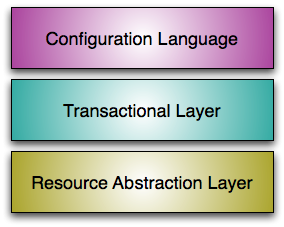
\includegraphics[width=0.5\textwidth]{images/layers.png}
\end{center}

\subsubsection{Configuration Language Layer}

The Configuration Language Layer is the Ruby API used to describe the desired state of the nodes. This layer exposes resources as Ruby methods. Because configurations are described in Ruby, it is possible to use the full power of Ruby metaprogramming to eliminate redundant code and integrate with other systems.

\begin{verbatim}
  user { 'dave':
    ensure     => present,
    uid        => '507',
    gid        => 'admin',
    shell      => '/bin/zsh'
  }
\end{verbatim}

The configuration language is platform independent, so that it can be used on any type of server that can be configured with puppet, and so that one configuration can be applied across heterogeneous systems.

This layer only concerns itself with the desired state of the nodes, it does not know how to communicate with other nodes in the system or realize the desired state.

\subsubsection{Transactional Layer}

\begin{center}
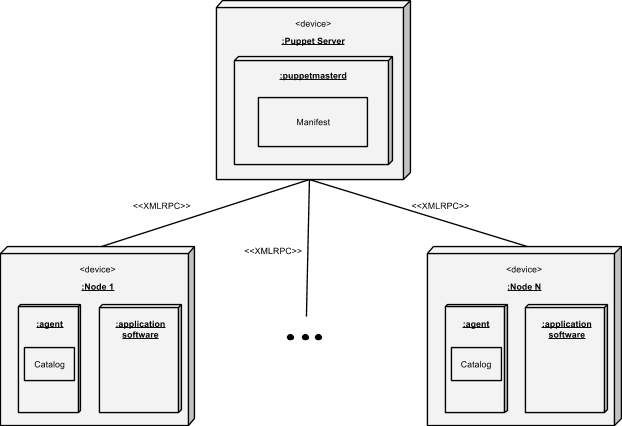
\includegraphics[width=\textwidth]{images/transaction-layer.png}
\end{center}

The Transactional Layer handles the communication between nodes in Puppet. This is crucial because the Puppet infrastructure contains many different agents which need not be on the same physical machine.

\begin{description}
\item[Puppet Master] The master coordinates the Puppet infrastructure. It has the canonical Manifests, queries facts from Puppet Nodes, processes these facts to build a catalog, sends that catalog to the nodes, and routes reports to the Report Collector. It can be thought of as an instance of the Mediator Pattern.
\item[Puppet Node] A node is a server who's software is managed by Puppet.
\item[Puppet Report Collector] A report collector receives information from one or more Puppet masters about the state of the system, which it makes available to software engineers.
\item[Development Machine] Software engineers may run the Puppet command line tool on their development machine to talk to the Puppet Master, among other tasks.
\end{description}

This layer may treat the configuration layer as a ``black box", it doesn't need to know what a particular configuration source file means, it just needs to transfer the information between agents. This layer does not know how to realize the desired state specified in the configuration layer; that is left to the Resource Abstraction Layer.

\subsubsection{Resource Abstraction Layer}

The Resource Abstraction Layer knows how to translate the instructions from the Configuration Language Layer into architecture-specific commands for nodes, Catalogs.

It relies upon the transactional layer to receive information from the Configuration Language and transfer Catalogs to their correct nodes.

\subsection{Logical View}

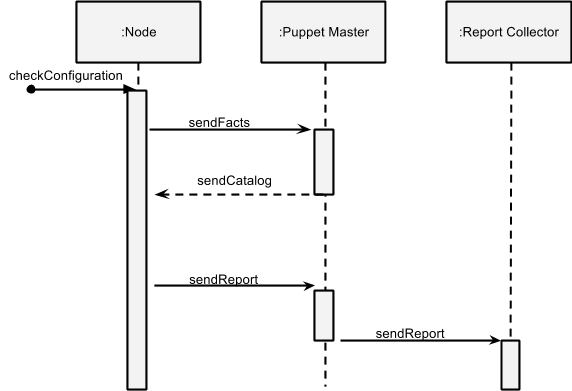
\includegraphics[width=\textwidth]{images/sequence-diagram.png}

The communication between the components is shown in the above sequence diagram. Each component is responsible for compiling the information required by the next step, so that clients are not accessing raw Puppet modules.

Periodically, (every 30 minutes by default) puppet nodes check their configuration with the puppet master. A module called ``Facter" gathers up information about the node, such as the operating system, IP address, or other custom information gathered by various Facter plugins. The node then sends this information on to the puppet master.

The puppet master uses the facts about the node together with the manifest files to compile a configuration specific to that node. The compiled configuration is called a catalog. The puppet master sends the catalog back to the node, which then applies the configuration. After the configuration has been applied, it generates a report of the configuration and sends it back to the puppet master. The puppet master then sends the report on to the report collector, which can either be puppet itself or a third party implementation based on puppet’s open API.

\section{Architectural Analysis}

% For each  quality attribute analysis  scenario, briefly discuss which design tactics and architectural styles or  patterns  (not  necessarily limited to those covered in  the lectures) have  been  applied to  address the attribute and relate the tactics, patterns or styles to the relevant architectural views.

\subsection{Reliability}

\textbf{An Apache webserver instance running on a server crashes. Puppet restarts Apache within a minute.}

Puppet Nodes periodically send ``facts", a snapshot of their state, to their Puppet Master. The Puppet Master compares these facts to the desired system state, as defined in the manifest, and creates a ``catalog" of changes to be made on the Puppet Node in order to bring it into the desired state.

In this case, the fact that Apache wasn't running would be reported to the Puppet Master. The Puppet Master would then send the node a catalog which would include commands to restart Apache.

The catalog can be thought of as a use of the command pattern.

\textbf{A software engineer wants to run Sendmail on a particular server node. She modifies the Manifest and pushes it to the Puppet Master. The Puppet Master is available and pushes these changes to the appropriate node within 30 minutes.}

The Puppet Master daemon is a single process that can be isolated from the rest of the infrastructure and carefully monitored. As long as the Puppet Master daemon is running and not reporting any errors, the rest of your infrastructure can be assumed to be working correctly.

In addition, it is possible to run multiple Puppet Masters, each collecting facts from and sending catalogs to a number of Puppet Nodes. This provides redundancy in case one Puppet Master fails.

\subsection{Modifiability / Maintainability}

\textbf{A software engineer wants to use Puppet to deploy new custom genetic analysis software. Different data sets will be deployed to different server nodes. She can easily extend Puppet's configuration language to represent these new types of configuration options.}

Puppet's Resource Abstraction Layer allows users to customize the configuration system used by Puppet to suit domain specific needs. This means that complex infrastructure deployed by Puppet will not be constrained by the expressiveness of Puppet's configuration language.

\subsection{Usability}

\textbf{A software engineer who just joined the team is tasked with setting up an FTP server on a node in the Company's infrastructure. She is quickly able to understand how Puppet works and perform the task.}

The Puppet Configuration language is based on Ruby, a well-known programming language widely considered to be  easy to use and powerful. Using Ruby as a user interface makes Puppet easy to learn, especially by people already framiliar with Ruby.

\section{Key Weaknesses} % (5  marks)

% Identify  and briefly discuss the main  weaknesses  of  the architecture. How
% could they  be  addressed?

Puppet is a complex system, often eschewing ease of use for modularity. Although the configuration language itself is easy to use, there is a steep learning curve for understanding the system as a whole. This is mitigated through good documentation and tutorials. Perhaps a graphical Puppet management interface would make the system even easier to use.

\section{References} % (1  mark)

% List  the references  to  the resources (books, papers, online  articles,
% etc.) you used  to  prepare this  report

\begin{itemize}
\item http://docs.puppetlabs.com/guides/introduction.html
\item http://docs.puppetlabs.com/learning/ral.html
\item http://puppetlabs.com/puppet/what-is-puppet
\item http://www.aosabook.org/en/puppet.html
\item http://www.slideshare.net/lkanies/portable-infrastructure-with-puppet
\end{itemize}

\end{document}
